\chapter{The Go Runtime On Bare Metal}

\begin{figure}[h]
\begin{center}
  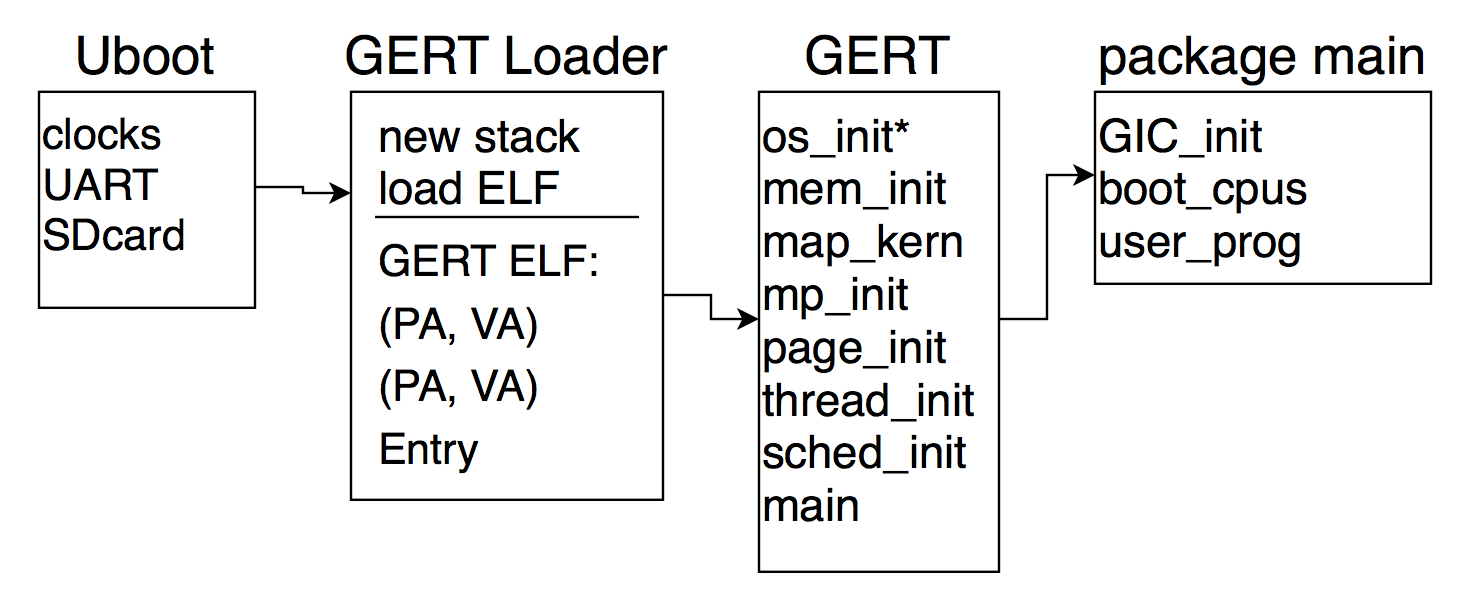
\includegraphics[scale=0.5]{boot_process}
\end{center}
  \caption{GERT Boot Process} \label{fig:boot}
\end{figure}

Even though Go code is compiled, it relies on a runtime to coordinate certain actions with the OS and support its concurrency model.
Timers, locks, and file descriptors are just a few of the OS abstractions that the runtime hinges on
in order to function at all. This means that getting compiled Go code to run bare metal on an SOC requires
more than just a boot loader, the Go runtime itself must be modified to work without any OS abstractions.
This poses a bootstrapping problem because any modifications made to the Go runtime's initialization
process must not inadvertently cause it to use an abstraction that does not yet exist. For example,
creating a new object with $make()$ during the boot process would be disasterous if the GC has not yet been initialized.
Modifying the Go runtime to boot on bare metal is tricky process because all additions should be made
in a non-destructive way that still preserves all of Go's useful primitives, including the standard library.


In observation of these constraints, GERT boots via a 3-step process as shown in  figure \ref{fig:boot}.
In step 1, u-boot is used to set up device clocks and load step 2 off of an SD card. Step 2 prepares the
Go stack with arguments and environment variables before jumping into GERT. Step 3 runs inside of GERT and it
finishes the boot process by initializing virtual memory, threading, and interrupt handlers.




%%The first stage is the u-boot
%%bootloader, a common bootloader for embedded devices, which
%%configures the clocks and loads the second stage off of an SD card. The second
%%stage bootloader is a small C program which contains the entire GERT kernel ELF in its data section. This stage sets
%%up the inital Go stack and loads the GERT ELF into memory before jumping to its entry point. The third stage
%%of the bootloader lives inside GERT and is mostly written in Go, along with some Plan 9 assembly. It finishes the
%%boot process by initializing virtual memory, threading, and additional cpus.



%%Working off the
%%initial stack from stage 2, the stage 3 bootloader enumerates all of RAM into page tables and creates an idenity mapping
%%with a new stack before turning on the MMU. After this, a thread scheduler is setup and synchronization primitives, like
%%$futex()$ are enabled. Additional CPU's are booted in main after the Go runtime has finished initializing.

%%\section{System Specification}
%%GERT is written on a Freescale i.MX6 Quad SOC which implements the (32 bit) ARMv7a Cortex A9 MPCore architecture.
%%The SOC sits on a Wandboard Quad baseboard. The i.MX6 Quad has 2GB of RAM and a wealth of memory mapped peripherals.
%%Look at the memory map below. The rest of this chapter will discuss the implementation details of booting and
%%running the Go runtime bare-metal on this SOC.
%%
%%<memory map of imx6 here>
%%
%%<memory map of GERT here>

\section{Step 1 Bring Up}
The u-boot loader is used to initialize device clocks and chain load the GERT bootloader.
Unlike desktop PCs, SOCs have no BIOS so it is entirely the programmer's job to initialize device clocks
and power on essential peripherals, such as the memory controller. U-boot is a simple bootloader which abstracts
this laborious process for all of the SOCs which it supports. GERT uses it to chain load its own, more specialized,
bootloader.

%%When the SOC is powered on, the program counter starts executing from ROM. The code in the ROM reads
%%u-boot into RAM and jumps into it. Unlike desktop PCs and laptops which use a BIOS to configure the
%%frequency dividers and RAM timings, the iMX6 has no such thing so u-boot does it instead.
%%U-boot programs the myriad of frequency dividers which are required
%%to run the i.MX6 at a frequency of 792MHz per core. After this, u-boot loads the GERT
%%kernel off the sdcard and into RAM at address 0x50000000. This address is specifically chosen because it
%%does not overlap with any ELF program headers of the GERT kernel which are loaded in stage 2. After
%%the stage 2 bootloader is in RAM, uboot jumps into it.

\section{Step 2 GERT Kernel Installation}
The GERT loader is a C program which sets up the initial Go stack and decompresses the Go kernel
ELF into RAM. GERT is compiled as a Linux Go program, so the Go runtime expects to find arguments
and environment variables in its initial stack. This is a convenient channel for passing
information, so the GERT loader gives the size of the GERT kernel as an input argument. GERT later uses this
size to determine its location in memory and initialize virtual memory.

The link address of the GERT binary must be also adjusted on a per-SOC basis in order for the Go
runtime to avoid using inaccessable memory. By default, Go links and loads at 0x0. This is a disaster
for most SOCs because they have reserved regions near that address. Fortunately, the Go compiler can
emit code at a different link addresses so this is not a significant problem.

%%Much like Linux, the kernel of GERT is wrapped in a custom
%%bootloader. This is necessary because GERT is compiled as a user space
%%Linux program which expects a stack and the standard ELF auxiliary vectors to be present on
%%startup.
%%
%%By default, the Go compiler links all programs at address 0x0. This would normally
%%be a disaster for the i.MX6 because the first megabyte of RAM is either inaccessable
%%or reserved for peripherals. One solution around this is to simply turn on the MMU
%%in the stage 2 bootloader but this creates a headache with preserving page tables
%%across the transition to Go. An alternative, and much simpler, solution is to
%%just change the link address of the Go ELF. This is the preferred approach so
%%GERT's build system uses a link address of 0x10000000 for the Go runtime, which is the start of
%%RAM on the iMX6. After loading the Go binary into RAM, the stage 2 bootloader reserves
%%4kb of initial stack and jumps into GERT.


\section{Step 3 Go Runtime Setup}

The Go runtime forms the basis of GERT's functionality but it is not equipped to
run on bare metal. The final steps of the boot process are accomplished in Go. GERT
initializes the minimum set of OS abstractions
which the Go runtime utilizes, before the runtime actually uses them. These abstractions are
virtual memory, thread scheduling, interrupt handling, timers, and booting secondary cores.

%%The thread scheduler and virtual memory system are statically initialized
%%in order to prevent Go runtime subsystems from running before the environment
%%is ready. At the beginning of execution, GERT is in a constrained
%%situation: Linux is not there but the Go runtime thinks it is. Specifically, there
%%is no scheduler, no virtual memory, no syscalls. Nothing but a 4kb stack
%%and the program counter. This is clearly inadequate for the Go runtime
%%to do anything but crash, so GERT creates all of these missing subsystems
%%,in Go, before the runtime actually uses them.


\subsection{Virtual Memory Setup}
\begin{figure}[h]
\begin{center}
  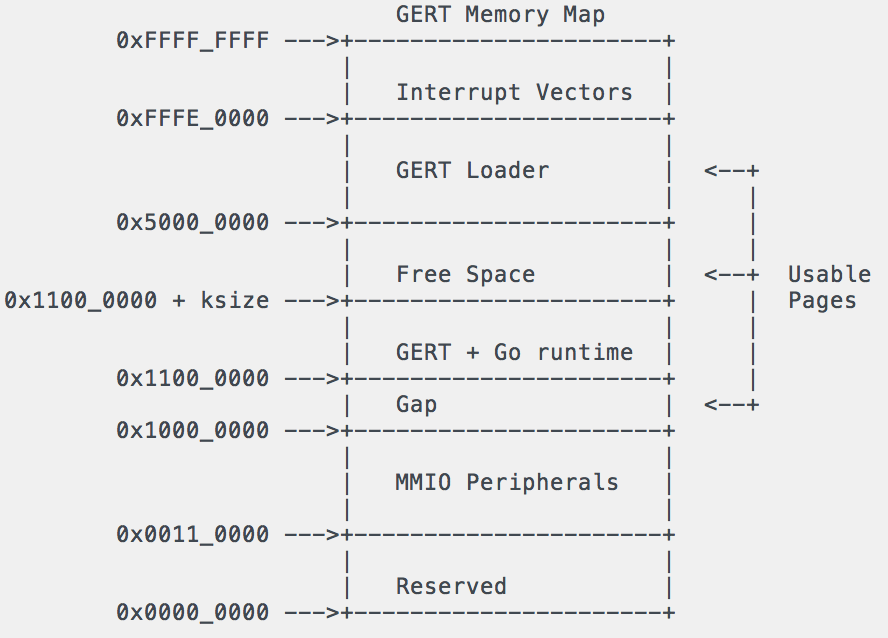
\includegraphics[scale=0.5]{gertmap}
\end{center}
  \caption{GERT Virtual Memory Layout} \label{fig:gertmap}
\end{figure}

GERT needs to have virtual memory because the Go runtime will readily use addreses that are within
reserved regions of physical memory. GERT still uses a single address space though because it has no concept
of user mode or kernel mode, so there is no need to switch page tables often. Additionally, the virtual memory
map changes infrequently because the Go runtime
only maps memory in big chunks. For these reasons, only 1MB pages are used and they are organized in a single
level table. The free pages are represented as a linked list so that map and unmap must only modify one link.
The memory layout in \ref{fig:gertmap} indicates the areas of memory that GERT can use as pages.
Notice how the GERT loader is recycled, freeing the space it previously used.

\subsection{Thread Scheduling and Trapframes}
\begin{figure}[h]
\begin{center}
  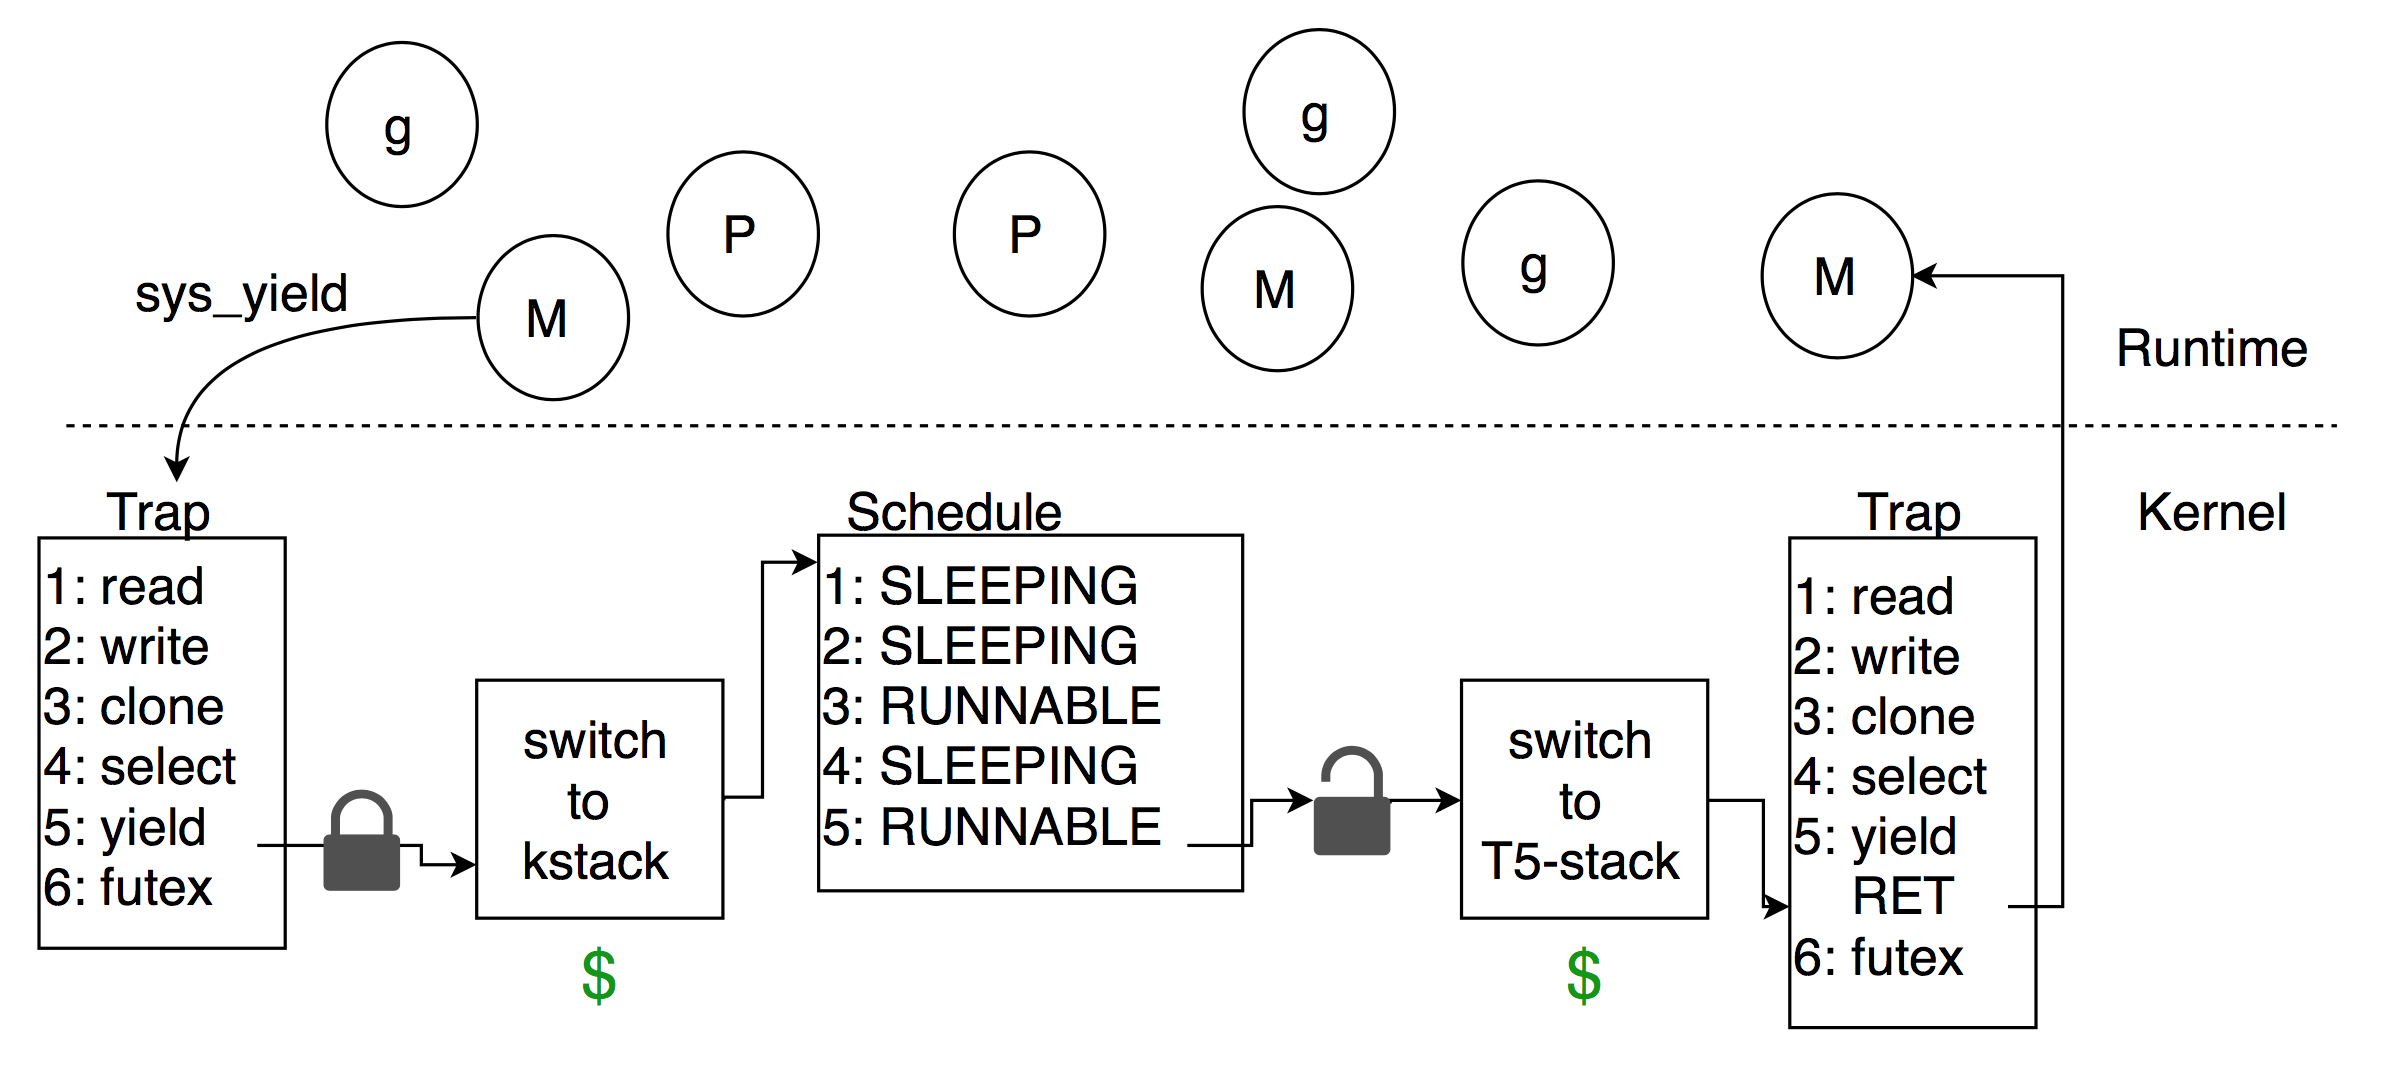
\includegraphics[scale=0.25]{syscall}
\end{center}
  \caption{Handling Go Runtime Syscalls} \label{fig:syscall}
\end{figure}

GERT models the entire Go runtime as a black box whose only entry and exit points
are through the syscalls it makes. This model is shown in \ref{fig:syscall}. To be clear, there is no such thing as a syscall in GERT.
Whenever the Go runtime makes a syscall, the processor mode is not changed and a new page table
is not installed. Instead, every instance of the syscall instruction in the Go runtime has been
replaced with a function call to $trap$. While execution is in $trap$, the Go runtime believes
that the OS is servicing its syscall, but in actuality the M is still running Go code inside
the GERT kernel. GERT maintains data structures that track the state of Go threads
outside the runtime's knowledge. It is important that all state inside the GERT kernel is
allocated outside the Go runtime's knowledge either with global variables or the kernel's
static memory allocator. If this constraint is not observed, then it is possible for the garbage collector
to potentially recycle memory from the kernel.

Each thread in GERT has an id, status, and trapframe associated with it (\ref{fig:threadtrap}).
The trap frame records the state of all the registers and the location of the stack at
the time that the Go runtime made a syscall.

\begin{figure}[h]
  \begin{lstlisting}
type thread_t struct {
	tf       trapframe
	state    uint32
	futaddr  uintptr
	sleeptil timespec
	id       uint32
}
type trapframe struct {
	lr  uintptr
	sp  uintptr
	fp  uintptr
	r0  uint32
	r1  uint32
	r2  uint32
	r3  uint32
	r10 uint32
}
\end{lstlisting}

  \caption{Thread state and Trapframes} \label{fig:threadtrap}
\end{figure}

The thread structure also contains a futex address, which is used by the runtime to wake
sleeping threads, and the time in the future to wake up if the thread is sleeping.

%%\begin{figure}[h]
%%  \begin{subfigure}[t!]{0.25\textwidth}
%%  \begin{lstlisting}
%%type thread_t struct {
%%	tf       trapframe
%%	state    uint32
%%	futaddr  uintptr
%%	sleeptil timespec
%%	id       uint32
%%	lock     Spinlock_t
%%}
%%\end{lstlisting}
%%  \end{subfigure}
%%  \begin{subfigure}[t!]{0.25\textwidth}
%%
%%  \begin{lstlisting}
%%type trapframe struct {
%%	lr  uintptr
%%	sp  uintptr
%%	fp  uintptr
%%	r0  uint32
%%	r1  uint32
%%	r2  uint32
%%	r3  uint32
%%	r10 uint32
%%}
%%\end{lstlisting}
%%
%%\end{subfigure}
%%  \caption{Thread state and Trapframes} \label{fig:threadtrap}
%%\end{figure}



\subsection{Interrupts}
\begin{figure}[h]
\begin{center}
  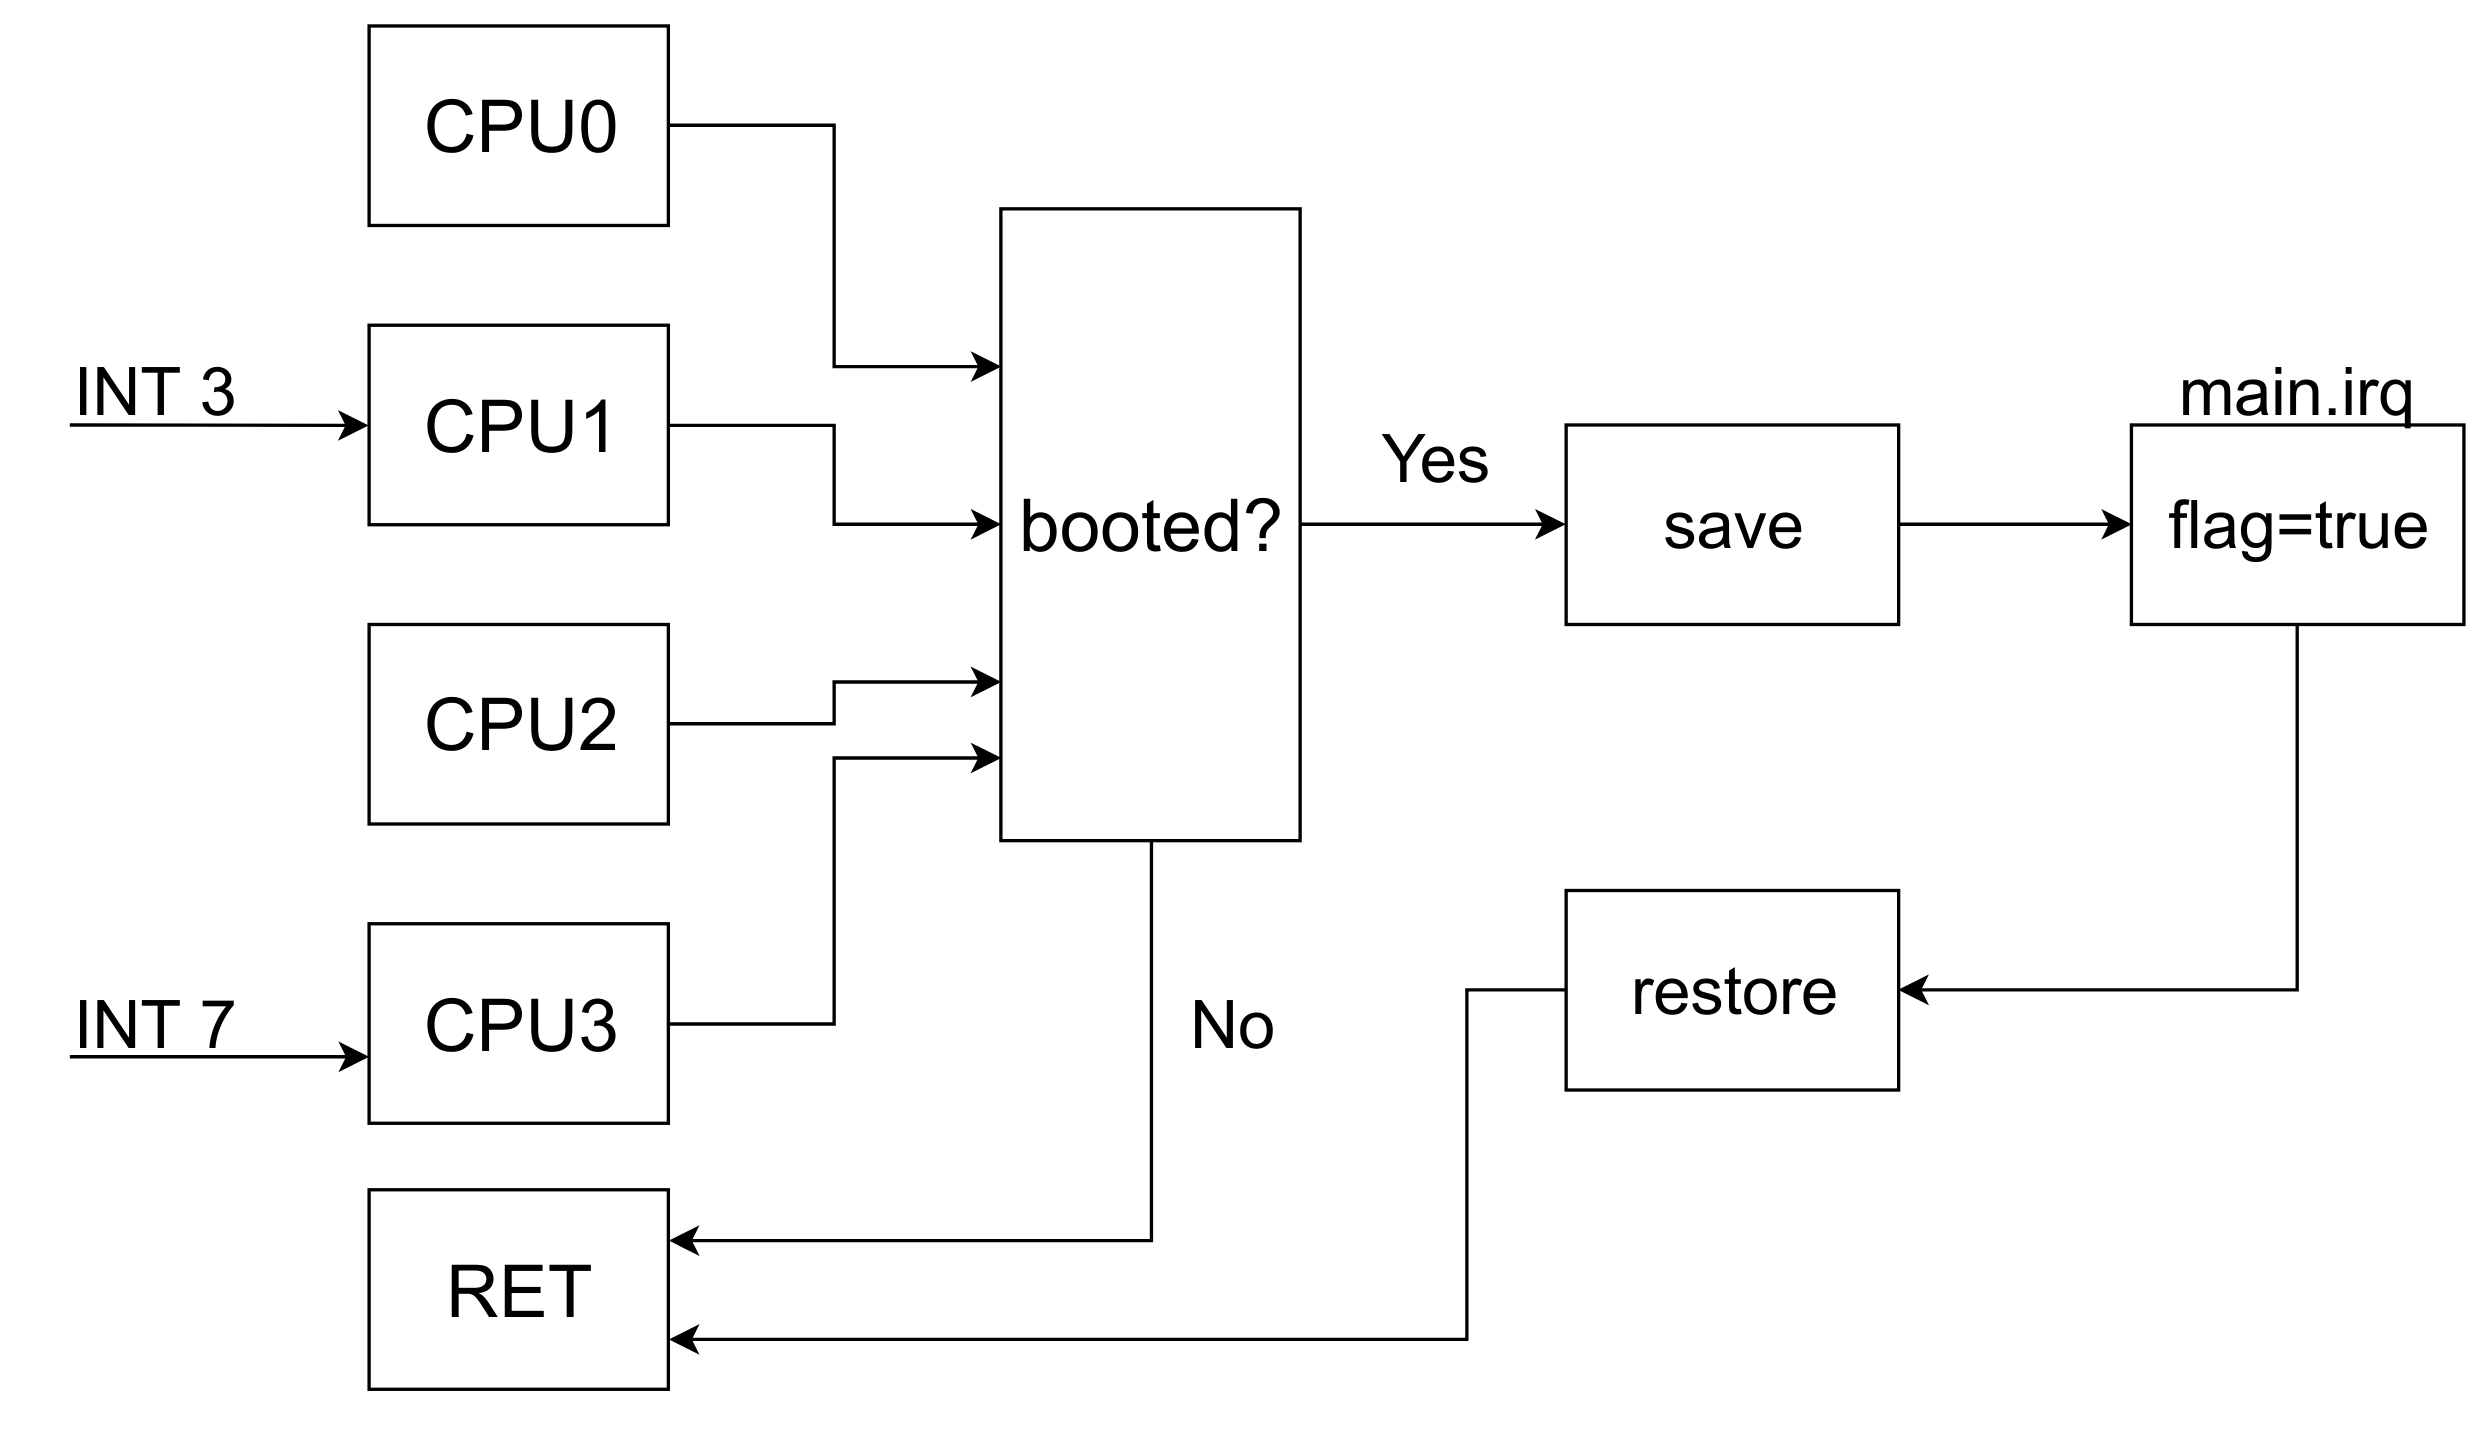
\includegraphics[scale=0.25]{interrupt}
\end{center}
  \caption{Handling Interrupts in GERT} \label{fig:interrupt}
\end{figure}



\subsection{Keeping Time}
\subsection{Booting Secondary CPUs}

